\documentclass[9pt,a4paper]{extarticle}
\usepackage{parskip}

% ======================
% Packages
% ======================
\usepackage[utf8]{inputenc}
\usepackage[T1]{fontenc}
\usepackage[brazil]{babel}
\usepackage{amsmath, amssymb}
\usepackage{amsthm}
\usepackage{geometry}
\usepackage{listings}
\usepackage{xcolor}
\usepackage{hyperref}
\usepackage{booktabs}
\usepackage{array}
\usepackage{tabularx}
\usepackage{enumitem}
\usepackage{microtype}
\usepackage{csquotes}
\usepackage{natbib}
\usepackage{graphicx}
\usepackage{tikz}

\usepackage{algorithm}
\usepackage{algpseudocode}

\definecolor{important}{RGB}{255, 100, 100}
\definecolor{notice}{RGB}{0, 102, 204}

\newcommand{\impt}[1]{\textcolor{important}{#1}}
\newcommand{\ntc}[1]{\textcolor{notice}{#1}}
\newcommand{\twodots}{\mathinner{\ldotp\ldotp}}

\setlist{nosep}
\geometry{margin=2cm}

% ======================
% Listings setup (Python)
% ======================
\definecolor{codebg}{rgb}{0.95,0.95,0.95}
\lstset{
    language=Python,
    backgroundcolor=\color{codebg},
    basicstyle=\ttfamily\footnotesize,
    keywordstyle=\color{blue},
    commentstyle=\color{gray},
    stringstyle=\color{red!70!black},
    showstringspaces=false,
    frame=single,
    breaklines=true,
    inputencoding=utf8
}

% ======================
% Document
% ======================
\begin{document}

\title{Divisão e Conquista \footnote{Material baseado em \citep{cormen2022algoritmos}}}
\author{PCC104 -- Projeto e ANálise de Algoritmos}
\date{\today}
\maketitle

\tableofcontents

% ==============================================================
\section{Introdução}

\textbf{Definição:} Divisão e conquista é uma técnica de projeto de algoritmos que resolve problemas de forma recursiva, seguindo três etapas:

\begin{enumerate}%[label=\textbf{\arabic*.}]
    \item \textbf{Dividir:} o problema original é dividido em subproblemas menores, que são instâncias menores do mesmo problema.

    \item \textbf{Conquistar:} os subproblemas são resolvidos recursivamente. Quando o subproblema é suficientemente pequeno, ele é resolvido
          diretamente (caso base).

    \item \textbf{Combinar:} as soluções dos subproblemas são combinadas para construir a solução do problema original.
\end{enumerate}

\subsection{Exemplo clássico - MergeSort}

\textbf{Merge Sort:} o arranjo é dividido ao meio, cada metade é ordenada recursivamente e, ao final, as duas metades ordenadas são combinadas em um único arranjo ordenado.

\begin{enumerate}
    \item \textbf{Dividir:} o arranjo de $n$ elementos é dividido em dois subarranjos de $n/2$ elementos cada.

    \item \textbf{Conquistar:} os dois subarranjos são ordenados recursivamente usando o próprio Merge Sort. Quando o subarranjo tem tamanho 1, ele já está trivialmente ordenado, esse é o caso base.

    \item \textbf{Combinar:} os dois subarranjos ordenados são intercalados (\textit{merged}) para produzir um único arranjo ordenado. Essa é a etapa central do algoritmo, onde ocorre o trabalho real.
\end{enumerate}

Comecemos pelo Combinar:

\begin{algorithm}[!ht]
\caption{Merge$(A, p, q, r)$}
\begin{algorithmic}[1]
\State $n_L = q - p + 1$  \Comment{tamanho do subarranjo esquerdo}
\State $n_R = r - q$       \Comment{tamanho do subarranjo direito}
\State seja $L[0 \,..\, n_L - 1]$ e $R[0 \,..\, n_R - 1]$ novos arranjos
\For{$i = 0$ \textbf{ to } $n_L - 1$}
    \State $L[i] = A[p + i]$
\EndFor
\For{$j = 0$ \textbf{ to } $n_R - 1$}
    \State $R[j] = A[q + j + 1]$
\EndFor
\State $i = 0$;\ $j = 0$;\ $k = p$
\While{$i < n_L$ \textbf{ and } $j < n_R$}
    \If{$L[i] \leq R[j]$}
        \State $A[k] = L[i]$;\ $i = i + 1$
    \Else
        \State $A[k] = R[j]$;\ $j = j + 1$
    \EndIf
    \State $k = k + 1$
\EndWhile
\While{$i < n_L$}
    \State $A[k] = L[i]$;\ $i = i + 1$;\ $k = k + 1$
\EndWhile
\While{$j < n_R$}
    \State $A[k] = R[j]$;\ $j = j + 1$;\ $k = k + 1$
\EndWhile
\end{algorithmic}
\end{algorithm}

\pagebreak 

Exemplo de execução do Merge:

\begin{figure}[!ht]
    \centering
    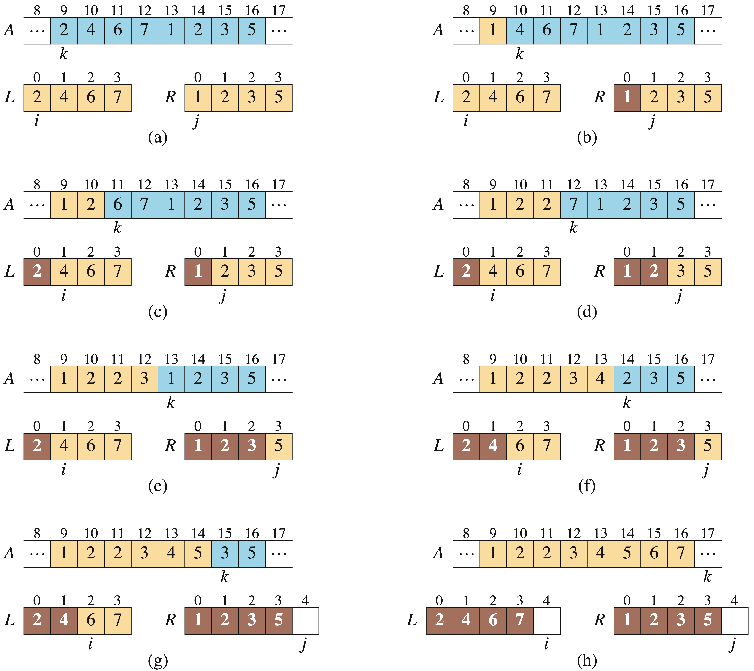
\includegraphics[width=0.75\textwidth]{Figure 2.3.pdf}
    \caption{Exemplo de execução do método Merge}
\end{figure}

Agora o método MergeSort

\begin{algorithm}[!ht]
\caption{MergeSort$(A, p, r)$}
\begin{algorithmic}[1]
\If{$p \geq r$}
    \State \Return
\EndIf
\State $q = \lfloor (p + r) / 2 \rfloor$
\State MergeSort$(A, p, q)$
\State MergeSort$(A, q + 1, r)$
\State Merge$(A, p, q, r)$
\end{algorithmic}
\end{algorithm}


Exemplo de execução do Merge:

\begin{figure}[!ht]
    \centering
    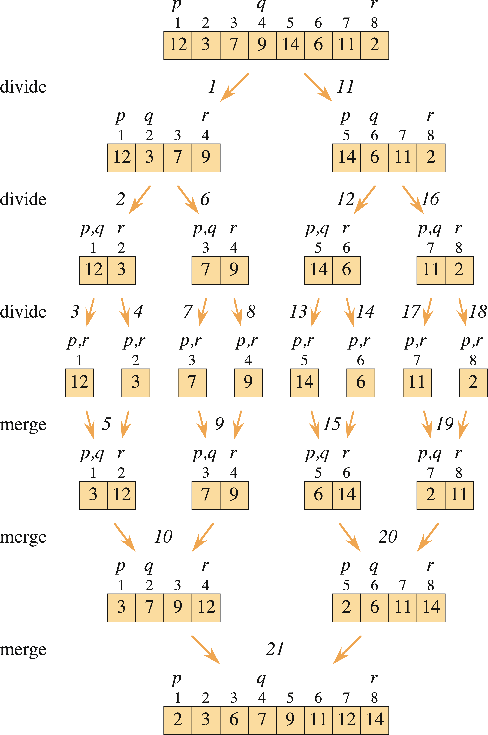
\includegraphics[width=0.5\textwidth]{Figure 2.4.pdf}
    \caption{Exemplo de execução do método MergeSort}
\end{figure}

\pagebreak

\subsection{Análise de Complexidade do Procedimento Merge}

Analisamos o custo de cada linha do procedimento \textsc{Merge}$(A, p, q, r)$, onde $n = r - p + 1$ denota o número total de elementos no subarranjo $A[p \twodots r]$ sendo intercalado, com $n_L = q - p + 1$ e $n_R = r - q$.

\begin{center}
\begin{tabular}{clcc}
\toprule
\textbf{Linha} & \textbf{Instrução} & \textbf{Custo} & \textbf{Vezes} \\
\midrule
1  & $n_L = q - p + 1$ & $c_1$ & $1$ \\
2  & $n_R = r - q$ & $c_2$ & $1$ \\
3  & aloca $L[0 \twodots n_L - 1]$ e $R[0 \twodots n_R - 1]$ & $c_3$ & $1$ \\
4  & \textbf{for} $i = 0$ \textbf{to} $n_L - 1$ & $c_4$ & $\displaystyle\sum_{i=0}^{n_L} 1$ \\
5  & \quad $L[i] = A[p + i]$ & $c_5$ & $\displaystyle\sum_{i=0}^{n_L - 1} 1$ \\
6  & \textbf{for} $j = 0$ \textbf{to} $n_R - 1$ & $c_6$ & $\displaystyle\sum_{j=0}^{n_R} 1$ \\
7  & \quad $R[j] = A[q + j + 1]$ & $c_7$ & $\displaystyle\sum_{j=0}^{n_R - 1} 1$ \\
8  & $i = 0$;\; $j = 0$;\; $k = p$ & $c_8$ & $1$ \\
9  & \textbf{while} $i < n_L$ \textbf{and} $j < n_R$ & $c_9$ & $\displaystyle\sum_{k=p}^{p+t} 1$ \\
10 & \quad \textbf{if} $L[i] \leq R[j]$ & $c_{10}$ & $\displaystyle\sum_{k=p}^{p+t-1} 1$ \\
11 & \quad\quad $A[k] = L[i]$;\; $i = i + 1$ & $c_{11}$ & $t_L$ \\
12 & \quad \textbf{else} & & \\
13 & \quad\quad $A[k] = R[j]$;\; $j = j + 1$ & $c_{12}$ & $t_R$ \\
14 & \quad $k = k + 1$ & $c_{13}$ & $\displaystyle\sum_{k=p}^{p+t-1} 1$ \\
15 & \textbf{while} $i < n_L$ & $c_{14}$ & $\displaystyle\sum_{i=t_L}^{n_L} 1$ \\
16 & \quad $A[k] = L[i]$;\; $i{=}i{+}1$;\; $k{=}k{+}1$ & $c_{15}$ & $\displaystyle\sum_{i=t_L}^{n_L - 1} 1$ \\
17 & \textbf{while} $j < n_R$ & $c_{16}$ & $\displaystyle\sum_{j=t_R}^{n_R} 1$ \\
18 & \quad $A[k] = R[j]$;\; $j{=}j{+}1$;\; $k{=}k{+}1$ & $c_{17}$ & $\displaystyle\sum_{j=t_R}^{n_R - 1} 1$ \\
\bottomrule
\end{tabular}
\end{center}

\noindent onde $t$ é o número de iterações do laço \textbf{while} principal (linha~9), $t_L$ é o número de vezes que um elemento de $L$ é copiado nesse laço, e $t_R = t - t_L$ é o número de vezes que um elemento de $R$ é copiado. Note que $t_L + t_R = t$.

O tempo total de execução é dado por:
\begin{align*}
T(n) &= c_1 + c_2 + c_3 + c_4(n_L + 1) + c_5 n_L + c_6(n_R + 1) + c_7 n_R + c_8 \\
     &\quad + c_9(t + 1) + c_{10}\, t + c_{11}\, t_L + c_{12}\, t_R + c_{13}\, t \\
     &\quad + c_{14}(n_L - t_L + 1) + c_{15}(n_L - t_L) \\
     &\quad + c_{16}(n_R - t_R + 1) + c_{17}(n_R - t_R)
\end{align*}

Observamos que cada um dos $n$ elementos é copiado para $A$ exatamente uma vez, seja no laço principal (linhas~11 ou~13), seja nos laços de finalização (linhas~16 ou~18). Portanto:
\[
t_L + (n_L - t_L) + t_R + (n_R - t_R) = n_L + n_R = n
\]

Agrupando os termos e simplificando, obtemos:
\[
T(n) = \alpha \cdot n + \beta
\]
onde $\alpha$ e $\beta$ são constantes que dependem dos custos $c_i$. Portanto:
\[
T(n) = \Theta(n)
\]

Concluímos que o procedimento \textsc{Merge} executa em tempo linear no número de elementos sendo intercalados. Este resultado é fundamental para a análise do \textsc{Merge-Sort}, cuja recorrência
\[
T(n) = 2\,T(n/2) + \Theta(n)
\]
resolve-se, pelo Teorema Mestre (caso~2, com $a = 2$, $b = 2$ e $f(n) = \Theta(n)$), para $T(n) = \Theta(n \lg n)$.

\section{Recorrências}

Uma \textbf{recorrência} é uma equação ou desigualdade que descreve uma função $T(n)$ em termos de seu valor em entradas menores. Recorrências surgem naturalmente quando um algoritmo divide um problema de tamanho $n$ em subproblemas menores, resolve-os recursivamente e combina as soluções.

Uma recorrência é composta por dois elementos essenciais:

O \textbf{caso recursivo} expressa $T(n)$ em função de valores $T(m)$ com $m < n$. Por exemplo, na recorrência do Merge-Sort, $T(n) = 2\,T(n/2) + \Theta(n)$ para $n > 1$, o caso recursivo captura o custo de resolver dois subproblemas de tamanho $n/2$ e intercalar os resultados em tempo $\Theta(n)$.

O \textbf{caso base} (ou \textbf{condição de contorno}) fornece o valor de $T(n)$ para entradas suficientemente pequenas, encerrando a recursão. No mesmo exemplo, $T(1) = \Theta(1)$, pois ordenar um único elemento tem custo constante. %Como o Cormen observa, as condições de contorno em geral são omitidas por conveniência, uma vez que para a maioria das recorrências algorítmicas elas afetam apenas as constantes ocultas na notação assintótica.

Uma recorrência é \textbf{bem definida} quando todo valor de $T(n)$ pode ser determinado de forma não ambígua: o caso recursivo sempre reduz o argumento em direção ao caso base, e o caso base está definido. Exemplos clássicos:
%
\[
T(n) = T(n-1) + c, \quad T(1) = c
\]
%
\noindent que descreve a busca linear e resolve-se para $T(n) = \Theta(n)$; e
%
\[
T(n) = 2\,T(n/2) + \Theta(n), \quad T(1) = \Theta(1)
\]
%
\noindent que descreve o Merge-Sort e resolve-se para $T(n) = \Theta(n \lg n)$.

Uma recorrência é \textbf{mal definida} quando o valor de $T(n)$ não pode ser determinado univocamente. Isso acontece, por exemplo, quando falta o caso base, como em $T(n) = 2\,T(n/2) + n$ sem nenhuma condição de contorno --- a solução fica indeterminada a menos de uma constante multiplicativa. Outro caso é quando o argumento não decresce em direção ao caso base, como $T(n) = T(n) + 1$, que não reduz o tamanho do problema e portanto não converge. Também pode ocorrer quando o domínio é ambíguo: a recorrência $T(n) = 2\,T(n/2) + n$ aplicada a $n$ ímpar requer uma convenção sobre o significado de $T(n/2)$ --- o Cormen resolve isso usando pisos e tetos, escrevendo $T(n) = T(\lfloor n/2 \rfloor) + T(\lceil n/2 \rceil) + \Theta(n)$, e depois mostra que essa distinção não afeta a ordem assintótica.


\section{Indução Matemática}

A \textbf{indução matemática} é uma técnica de prova utilizada para demonstrar que uma proposição $P(n)$ vale para todo número natural $n \geq n_0$, onde $n_0$ é um valor base. O método de substituição para resolver recorrências, apresentado na seção seguinte, depende diretamente desta técnica, de modo que sua compreensão é pré-requisito essencial.

\subsection{Estrutura da Prova por Indução}

Uma prova por indução é composta por dois passos:

\begin{enumerate}
    \item \textbf{Caso base.} Verificar que $P(n_0)$ é verdadeira para algum valor inicial $n_0$.
    \item \textbf{Passo indutivo.} Assumir que $P(k)$ é verdadeira para algum $k \geq n_0$ (esta suposição é chamada de \textbf{hipótese indutiva}) e, a partir dela, provar que $P(k+1)$ também é verdadeira.
\end{enumerate}

\noindent Se ambos os passos são satisfeitos, concluímos que $P(n)$ vale para todo $n \geq n_0$. A intuição é a de um efeito dominó: o caso base derruba a primeira peça, e o passo indutivo garante que cada peça derruba a seguinte.

\subsection{Exemplo: Soma dos Primeiros $n$ Naturais}

Demonstremos que, para todo $n \geq 1$,
%
\[
P(n): \quad \sum_{i=1}^{n} i = \frac{n(n+1)}{2}.
\]

\textbf{Caso base.} Para $n = 1$, o lado esquerdo vale $\sum_{i=1}^{1} i = 1$ e o lado direito vale $1 \cdot 2 / 2 = 1$. Logo $P(1)$ é verdadeira.

\textbf{Passo indutivo.} Suponha que $P(k)$ é verdadeira, isto é, $\sum_{i=1}^{k} i = k(k+1)/2$. Queremos provar que $P(k+1)$ vale. Temos:
%
\begin{align*}
\sum_{i=1}^{k+1} i &= \left(\sum_{i=1}^{k} i\right) + (k+1) \\
                    &= \frac{k(k+1)}{2} + (k+1) \\
                    &= \frac{k(k+1) + 2(k+1)}{2} \\
                    &= \frac{(k+1)(k+2)}{2}
\end{align*}
%
\noindent que é exatamente a fórmula avaliada em $n = k+1$. Portanto $P(k+1)$ é verdadeira, e por indução $P(n)$ vale para todo $n \geq 1$. \qed

\subsection{Indução Forte}

Na \textbf{indução forte} (ou \textbf{indução completa}), a hipótese indutiva é mais poderosa: em vez de assumir apenas que $P(k)$ vale, assumimos que $P(m)$ vale para \emph{todo} $m$ com $n_0 \leq m \leq k$, e a partir disso provamos $P(k+1)$.

Essa variante é logicamente equivalente à indução simples, mas em muitas situações é mais conveniente. Em particular, o método de substituição para recorrências utiliza indução forte, pois o valor de $T(n)$ pode depender de $T$ avaliada em múltiplas entradas menores --- como $T(\lfloor n/2 \rfloor)$ e $T(\lceil n/2 \rceil)$ simultaneamente --- e precisamos que a hipótese valha para todas elas, não apenas para $T(n-1)$.

\subsection{Exemplo com Indução Forte}

Demonstremos que, para todo $n \geq 1$, todo inteiro $n \geq 2$ pode ser escrito como produto de números primos.

\textbf{Caso base.} Para $n = 2$, o próprio $2$ é primo, logo é trivialmente um produto de primos.

\textbf{Passo indutivo.} Suponha que, para todo $m$ com $2 \leq m \leq k$, $m$ pode ser escrito como produto de primos. Considere $k + 1$. Se $k + 1$ é primo, a afirmação é imediata. Se $k + 1$ não é primo, então existem inteiros $a, b$ com $2 \leq a, b \leq k$ tais que $k + 1 = a \cdot b$. Pela hipótese indutiva (que vale para todo $m \leq k$), ambos $a$ e $b$ podem ser escritos como produto de primos, e portanto $k + 1 = a \cdot b$ também pode. \qed

Note que a indução simples não seria suficiente aqui: saber que $k$ é produto de primos nada diz sobre a fatoração de $k+1$.

\subsection{Indução e Recorrências}

A conexão entre indução e recorrências é direta. Provar que $T(n) \leq c\,g(n)$ para uma recorrência é essencialmente uma prova por indução forte: assumimos que $T(m) \leq c\,g(m)$ para todo $m < n$, substituímos na recorrência, e verificamos que $T(n) \leq c\,g(n)$ segue algebricamente. O caso base corresponde a verificar a desigualdade para valores pequenos de $n$, possivelmente escolhendo a constante $c$ grande o suficiente para acomodá-los. Esta é precisamente a mecânica do \textbf{método de substituição}, que será desenvolvido na próxima seção.

\section{Método de Substituição}

O \textbf{método de substituição} para resolver recorrências, conforme apresentado no Cormen (CLRS), consiste em dois passos: (1)~conjecturar a forma da solução e (2)~usar indução matemática para provar que a conjectura está correta, determinando as constantes apropriadas.

\subsection{Estrutura do Método}

Suponha que desejamos resolver uma recorrência $T(n)$. O método procede da seguinte forma:

\begin{enumerate}
    \item \textbf{Conjecturar} um limitante da forma $T(n) \leq c \cdot g(n)$ (para um limitante superior) ou $T(n) \geq c \cdot g(n)$ (para um limitante inferior), onde $g(n)$ é a função candidata e $c > 0$ é uma constante a ser determinada.
    \item \textbf{Provar por indução} que a conjectura vale para todo $n$ suficientemente grande, assumindo que ela vale para entradas menores.
\end{enumerate}

\subsection{Exemplo: Recorrência do Merge-Sort}

Considere a recorrência
%
\[
T(n) = 2\,T(\lfloor n/2 \rfloor) + dn
\]
%
\noindent com $T(1) = \Theta(1)$ e $d > 0$ uma constante que reflete o custo linear do procedimento \textsc{Merge}. Conjecturamos que $T(n) = O(n \lg n)$, ou seja, que existe uma constante $c > 0$ tal que $T(n) \leq c\,n\lg n$ para todo $n \geq n_0$.

\textbf{Passo indutivo.} Assumimos, por indução forte, que $T(m) \leq c\,m\lg m$ para todo $m < n$. Em particular, $T(\lfloor n/2 \rfloor) \leq c\,\lfloor n/2 \rfloor \lg \lfloor n/2 \rfloor$. Substituindo na recorrência:
%
\begin{align*}
T(n) &\leq 2\bigl(c\,\lfloor n/2 \rfloor \lg \lfloor n/2 \rfloor\bigr) + dn \\
     &\leq c\,n\lg(n/2) + dn \\
     &= c\,n\lg n - c\,n + dn \\
     &= c\,n\lg n - (c - d)\,n \\
     &\leq c\,n\lg n
\end{align*}
%
\noindent onde a última desigualdade vale desde que $c \geq d$, pois nesse caso $(c - d)\,n \geq 0$.

\textbf{Caso base.} Seja $T(1) = a$ para alguma constante $a > 0$. Para $n = 1$, a conjectura exigiria $T(1) \leq c \cdot 1 \cdot \lg 1 = 0$, o que falha. Para $n = 2$, temos $T(2) = 2\,T(1) + 2d = 2a + 2d$. Precisamos que $T(2) \leq c \cdot 2 \lg 2 = 2c$, o que vale para $c \geq a + d$. Portanto, tomando $n_0 = 2$ e $c \geq a + d \geq d$, ambas as condições --- do caso base e do passo indutivo --- são satisfeitas simultaneamente.

Concluímos que $T(n) \leq c\,n\lg n$ para todo $n \geq 2$, e assim $T(n) = O(n \lg n)$.

\subsection{Flexibilidade na Escolha do Caso Base}

Ao aplicar o método de substituição, é comum que a conjectura $T(n) \leq c\,g(n)$ falhe para valores pequenos de $n$. Isso não invalida a prova, desde que a indução seja iniciada a partir de um $n_0$ adequado. O Cormen (CLRS) dedica atenção explícita a este ponto, pois ele é fonte frequente de confusão.

\subsubsection{Por que a Falha em $n = 1$ Não É Problema}

Recordemos que a notação assintótica $T(n) = O(g(n))$ exige apenas que $T(n) \leq c\,g(n)$ para todo $n \geq n_0$, onde tanto $c$ quanto $n_0$ são constantes que podemos escolher. Não há obrigação de que a desigualdade valha para \emph{todo} $n$; basta que valha a partir de algum ponto.

No exemplo da recorrência do Merge-Sort, a conjectura $T(n) \leq c\,n\lg n$ falha para $n = 1$ porque $\lg 1 = 0$, de modo que o lado direito se anula independentemente de $c$. Contudo, isso reflete apenas a inadequação da função $n \lg n$ como limitante para $n = 1$, e não uma falha da conjectura assintótica.

\subsubsection{A Justificativa Formal}

A prova por indução forte requer dois ingredientes: que $T(n) \leq c\,g(n)$ valha para todos os valores de $n$ em um intervalo base $[n_0, \ldots, n_1]$ suficiente para ancorar a indução, e que o passo indutivo preserve a desigualdade para todo $n > n_1$. O intervalo base precisa cobrir todos os valores que a recorrência pode atingir antes de se reduzir a subproblemas já tratados pelo passo indutivo.

No caso de $T(n) = 2\,T(\lfloor n/2 \rfloor) + dn$, qualquer $n \geq 2$ gera subproblemas de tamanho $\lfloor n/2 \rfloor \geq 1$. Se tomamos $n_0 = 2$, o menor subproblema que o passo indutivo precisa consultar é $T(1)$, que não está coberto pela hipótese. Porém, como $T(1)$ é uma constante conhecida --- digamos $T(1) = a$ --- podemos incorporá-la diretamente na verificação do caso base para $n = 2$:
%
\[
T(2) = 2a + 2d \leq 2c = c \cdot 2 \lg 2
\]
%
\noindent que vale para $c \geq a + d$. A partir daí, todo $n \geq 3$ gera subproblemas de tamanho $\lfloor n/2 \rfloor \geq 2$, e o passo indutivo se aplica normalmente.

\subsubsection{A Observação do Cormen}

O Cormen formaliza esta flexibilidade da seguinte maneira: como a notação assintótica só exige que a desigualdade valha para $n \geq n_0$, podemos substituir as condições de contorno da recorrência --- que tipicamente cobrem um número finito e constante de valores --- pela escolha de $c$ suficientemente grande para acomodá-las. Um número finito de condições da forma $T(n_i) \leq c\,g(n_i)$ pode sempre ser satisfeito tomando $c \geq \max_i \{T(n_i)/g(n_i)\}$, desde que $g(n_i) > 0$ para cada $n_i$ no intervalo base.

Isso significa, na prática, que ao aplicar o método de substituição podemos nos concentrar no passo indutivo --- que é onde a estrutura da recorrência é explorada --- e tratar o caso base como uma verificação técnica, ajustando $c$ e $n_0$ ao final da prova.

\subsection{Armadilhas Comuns}

O Cormen destaca algumas armadilhas frequentes ao aplicar o método de substituição:

A primeira é \textbf{errar na forma da hipótese indutiva}. Por exemplo, ao tentar provar que $T(n) = 2\,T(\lfloor n/2 \rfloor) + n$ é $O(n)$, assumimos $T(\lfloor n/2 \rfloor) \leq c\,\lfloor n/2 \rfloor$ e obtemos $T(n) \leq c\,n + n = (c+1)\,n$, o que \emph{não} prova $T(n) \leq c\,n$ para a \emph{mesma} constante $c$. A indução falha porque o termo residual $n$ impede que a hipótese se ``feche''.

A segunda é a necessidade de, em certos casos, \textbf{subtrair um termo de ordem inferior} na hipótese indutiva para que a prova funcione. Por exemplo, para a recorrência $T(n) = T(\lfloor n/2 \rfloor) + T(\lceil n/2 \rceil) + 1$, a conjectura $T(n) \leq c\,n$ não fecha diretamente. No entanto, conjecturar $T(n) \leq c\,n - d$ para constantes $c, d > 0$ fornece a margem necessária para absorver o termo constante e completar a indução.

\subsection{Como Obter Boas Conjecturas}

O Cormen sugere algumas heurísticas para formular a conjectura inicial. Se a recorrência é semelhante a uma já conhecida, pode-se usar a mesma forma: por exemplo, $T(n) = 2\,T(\lfloor n/2 \rfloor + 17) + n$ provavelmente tem solução $O(n \lg n)$, pois o termo aditivo $17$ torna-se insignificante para $n$ grande. Outra estratégia é provar limitantes frouxos --- primeiro $O(n^2)$ e $\Omega(n)$ --- e ir refinando progressivamente até que os limitantes superior e inferior coincidam. Finalmente, pode-se usar a \textbf{árvore de recursão} (apresentada na próxima seção) como ferramenta para gerar uma boa conjectura, que depois é verificada rigorosamente pelo método de substituição.

\section{Método da Árvore de Recursão}

O \textbf{método da árvore de recursão} é uma técnica para resolver recorrências que consiste em expandir a recorrência em uma árvore cujos nós representam os custos incorridos em cada nível de recursão. Somando os custos de todos os níveis, obtém-se uma expressão para o custo total, que pode ser usada diretamente como solução ou como conjectura a ser verificada rigorosamente pelo método de substituição. O Cormen (CLRS) apresenta a árvore de recursão tanto como ferramenta heurística para gerar boas conjecturas quanto, quando conduzida com cuidado suficiente, como prova direta.

\subsection{Construção da Árvore}

Considere uma recorrência da forma geral
%
\[
T(n) = a\,T(n/b) + f(n)
\]
%
\noindent com caso base $T(1) = \Theta(1)$. A árvore de recursão é construída da seguinte maneira:

\begin{enumerate}
    \item A \textbf{raiz} contém o custo $f(n)$, correspondente ao trabalho realizado fora das chamadas recursivas.
    \item Cada nó interno com custo relativo a um subproblema de tamanho $m$ gera $a$ filhos, cada um associado a um subproblema de tamanho $m/b$.
    \item As \textbf{folhas} correspondem ao caso base, cada uma contribuindo com custo $\Theta(1)$.
\end{enumerate}

\noindent O custo total é então a soma dos custos de todos os nós, que pode ser organizada nível a nível.

\subsection{Exemplo: Recorrência do Merge-Sort}

Considere a recorrência
%
\[
T(n) = 2\,T(n/2) + dn
\]
%
\noindent com $T(1) = a$. A árvore tem a seguinte estrutura:

\begin{center}
\begin{tikzpicture}[
    level distance=1.4cm,
    sibling distance=1.2cm,
    every node/.style={},
    edge from parent/.style={draw, -},
    level 1/.style={sibling distance=5cm},
    level 2/.style={sibling distance=2.5cm},
    level 3/.style={sibling distance=1.2cm},
    cost/.style={anchor=west, xshift=1.5cm},
]

% Rótulo de nível
\node[anchor=east, xshift=-3.5cm] at (-2,0) {\footnotesize Nível 0};
\node[anchor=east, xshift=-3.5cm] at (-2,-1.4) {\footnotesize Nível 1};
\node[anchor=east, xshift=-3.5cm] at (-2,-2.8) {\footnotesize Nível 2};
\node[anchor=east, xshift=-3.5cm] at (-2,-4.2) {\footnotesize Nível $\lg n$};

% Custo por nível
\node[anchor=west, xshift=4.5cm] at (1,0) {$dn$};
\node[anchor=west, xshift=4.5cm] at (1,-1.4) {$dn$};
\node[anchor=west, xshift=4.5cm] at (1,-2.8) {$dn$};
\node[anchor=west, xshift=4.5cm] at (1,-4.2) {$an$};

% Árvore
\node {$dn$}
    child {node {$d\dfrac{n}{2}$}
        child {node {$d\dfrac{n}{4}$}
            child {node[yshift=-0.4cm] {$a$} edge from parent[dashed]}
            child {node[yshift=-0.4cm] {$a$} edge from parent[dashed]}
        }
        child {node {$d\dfrac{n}{4}$}
            child {node[yshift=-0.4cm] {$a$} edge from parent[dashed]}
            child {node[yshift=-0.4cm] {$a$} edge from parent[dashed]}
        }
    }
    child {node {$d\dfrac{n}{2}$}
        child {node {$d\dfrac{n}{4}$}
            child {node[yshift=-0.4cm] {$a$} edge from parent[dashed]}
            child {node[yshift=-0.4cm] {$a$} edge from parent[dashed]}
        }
        child {node {$d\dfrac{n}{4}$}
            child {node[yshift=-0.4cm] {$a$} edge from parent[dashed]}
            child {node[yshift=-0.4cm] {$a$} edge from parent[dashed]}
        }
    };

% Pontos verticais entre nível 2 e folhas
\node at (0,-3.5) {$\vdots$};

\end{tikzpicture}
\end{center}

\noindent No nível $i$, há $2^i$ nós, cada um com custo $d(n/2^i)$, de modo que o custo total do nível é $2^i \cdot d(n/2^i) = dn$. A recursão atinge o caso base quando $n/2^i = 1$, isto é, quando $i = \lg n$. Portanto a árvore tem $\lg n + 1$ níveis (de $0$ a $\lg n$). No último nível há $2^{\lg n} = n$ folhas, cada uma com custo $a$, totalizando $an$.

O custo total é a soma dos custos de todos os níveis:
%
\[
T(n) = \underbrace{dn + dn + \cdots + dn}_{\lg n \text{ parcelas}} + an = dn\lg n + an
\]
%
\noindent e portanto $T(n) = \Theta(n \lg n)$.

\subsection{Exemplo: Recorrência com Subproblemas Desiguais}

Considere agora a recorrência
%
\[
T(n) = T(n/3) + T(2n/3) + dn
\]
%
\noindent que surge quando um algoritmo de divisão e conquista particiona o problema de forma desbalanceada.

\begin{figure}[!ht]
    \centering
    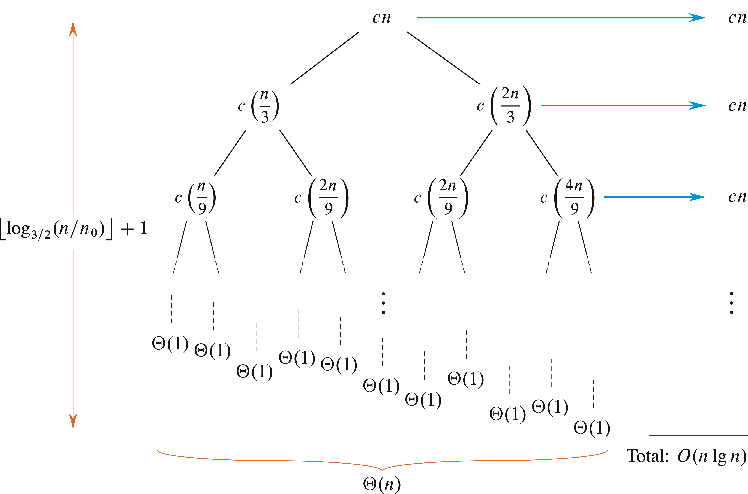
\includegraphics[width=0.8\textwidth]{Figure 4.2.pdf}
\end{figure}

\noindent A árvore não é completa: o ramo esquerdo reduz o tamanho por um fator de $3$, atingindo o caso base no nível $\log_3 n$, enquanto o ramo direito reduz por um fator de $3/2$, atingindo o caso base no nível $\log_{3/2} n$. Apesar da assimetria, o custo de cada nível completo é no máximo $dn$, pois os tamanhos dos subproblemas em qualquer nível somam no máximo $n$. O caminho mais longo da raiz a uma folha tem comprimento $\log_{3/2} n$, de modo que a árvore tem no máximo $\log_{3/2} n + 1$ níveis. Portanto:
%
\[
T(n) \leq dn \cdot (\log_{3/2} n + 1) = O(n \lg n)
\]
%
\noindent onde usamos que $\log_{3/2} n = \Theta(\lg n)$, pois a mudança de base introduz apenas um fator constante. Para confirmar que $T(n) = \Omega(n \lg n)$, basta observar que o caminho mais curto tem comprimento $\log_3 n = \Theta(\lg n)$ e que cada um desses níveis contribui com custo exatamente $dn$. Concluímos que $T(n) = \Theta(n \lg n)$.

Como o Cormen observa, este é um caso em que a árvore de recursão é especialmente útil: a recorrência não se enquadra diretamente na forma $T(n) = a\,T(n/b) + f(n)$ com subproblemas de tamanho igual, mas a árvore fornece uma conjectura precisa que pode ser verificada pelo método de substituição.

\subsection{Exemplo: Custo Geométrico por Nível}

Considere a recorrência
%
\[
T(n) = 3\,T(n/4) + dn^2
\]

\begin{figure}[!ht]
    \centering
    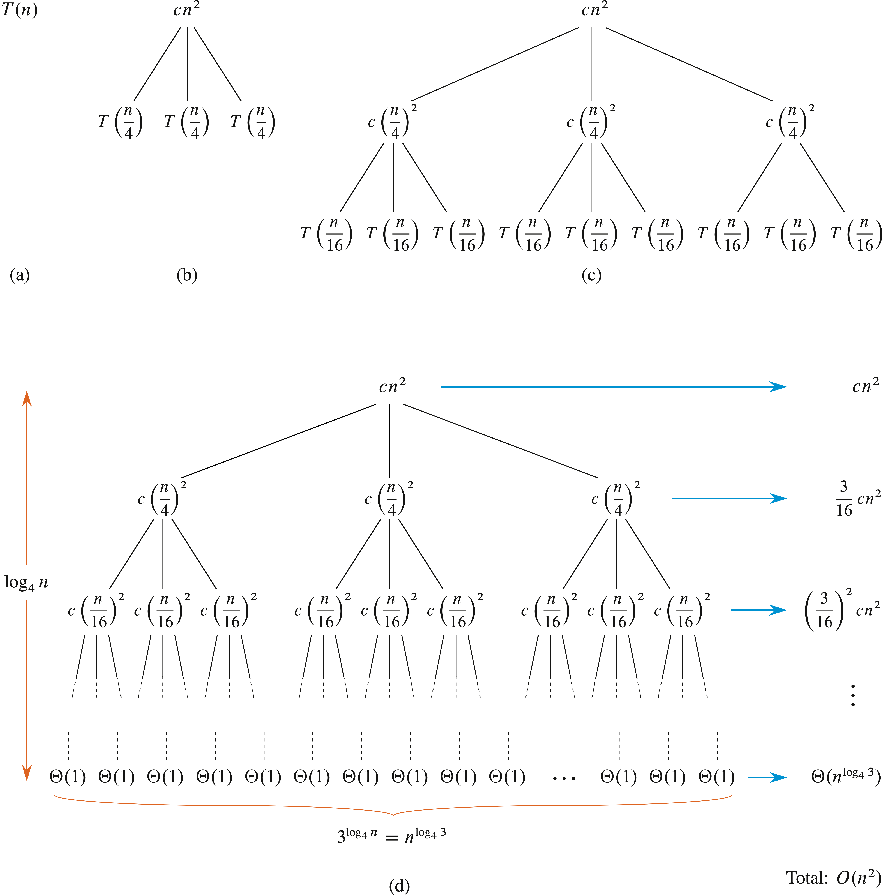
\includegraphics[width=0.8\textwidth]{Figure 4.1.pdf}
\end{figure}

\noindent Neste caso, cada nível da árvore tem um custo diferente. No nível $i$, há $3^i$ nós, cada um com custo $d(n/4^i)^2$, de modo que o custo total do nível é $3^i \cdot d(n/4^i)^2 = \left(\frac{3}{16}\right)^i dn^2$. A profundidade da árvore é $\log_4 n$, pois o caso base é atingido quando $n/4^i = 1$. A soma dos custos por nível forma uma série geométrica:
%
\[
T(n) = dn^2 \sum_{i=0}^{\log_4 n - 1} \left(\frac{3}{16}\right)^i + \Theta\!\left(n^{\log_4 3}\right)
\]
%
\noindent onde o último termo corresponde ao custo das $3^{\log_4 n} = n^{\log_4 3}$ folhas. Como a razão $3/16 < 1$, a série geométrica converge, e obtemos:
%
\[
\sum_{i=0}^{\log_4 n - 1} \left(\frac{3}{16}\right)^i < \sum_{i=0}^{\infty} \left(\frac{3}{16}\right)^i = \frac{1}{1 - 3/16} = \frac{16}{13}
\]
%
\noindent Portanto $T(n) \leq \frac{16}{13}\,dn^2 + \Theta(n^{\log_4 3}) = O(n^2)$, pois $\log_4 3 < 1 < 2$. O custo é dominado pelo nível da raiz, que é o cenário típico quando $f(n)$ cresce mais rápido que o número de subproblemas --- uma situação que será formalizada pelo caso~3 do Teorema Mestre.

\subsection{Árvore de Recursão como Conjectura}

O Cormen enfatiza que a árvore de recursão é, em muitos casos, utilizada como ferramenta heurística: ela fornece uma conjectura para a forma assintótica de $T(n)$, que deve ser verificada rigorosamente pelo método de substituição. No entanto, quando a análise é conduzida com cuidado --- somando corretamente todos os níveis e tratando pisos, tetos e casos base --- a própria árvore constitui uma prova válida.


\section{Método da Árvore de Recursão}

O \textbf{método da árvore de recursão} é uma técnica para resolver recorrências que consiste em expandir a recorrência em uma árvore cujos nós representam os custos incorridos em cada nível de recursão. Somando os custos de todos os níveis, obtém-se uma expressão para o custo total, que pode ser usada diretamente como solução ou como conjectura a ser verificada rigorosamente pelo método de substituição. O Cormen (CLRS) apresenta a árvore de recursão tanto como ferramenta heurística para gerar boas conjecturas quanto, quando conduzida com cuidado suficiente, como prova direta.

\subsection{Construção da Árvore}

Considere uma recorrência da forma geral
%
\[
T(n) = a\,T(n/b) + f(n)
\]
%
\noindent com caso base $T(1) = \Theta(1)$. A árvore de recursão é construída da seguinte maneira:

\begin{enumerate}
    \item A \textbf{raiz} contém o custo $f(n)$, correspondente ao trabalho realizado fora das chamadas recursivas.
    \item Cada nó interno com custo relativo a um subproblema de tamanho $m$ gera $a$ filhos, cada um associado a um subproblema de tamanho $m/b$.
    \item As \textbf{folhas} correspondem ao caso base, cada uma contribuindo com custo $\Theta(1)$.
\end{enumerate}

\noindent O custo total é então a soma dos custos de todos os nós, que pode ser organizada nível a nível.

\subsection{Exemplo: Recorrência do Merge-Sort}

Considere a recorrência
%
\[
T(n) = 2\,T(n/2) + dn
\]
%
\noindent com $T(1) = a$. A árvore tem a seguinte estrutura:

\begin{itemize}
    \item \textbf{Nível 0:} um único nó com custo $dn$. Há $1 = 2^0$ subproblema de tamanho $n/2^0 = n$.
    \item \textbf{Nível 1:} dois nós, cada um com custo $d(n/2)$. O custo total do nível é $2 \cdot d(n/2) = dn$.
    \item \textbf{Nível 2:} quatro nós, cada um com custo $d(n/4)$. O custo total do nível é $4 \cdot d(n/4) = dn$.
    \item \textbf{Nível $i$:} há $2^i$ nós, cada um com custo $d(n/2^i)$. O custo total do nível é $2^i \cdot d(n/2^i) = dn$.
\end{itemize}

\noindent A recursão atinge o caso base quando $n/2^i = 1$, isto é, quando $i = \lg n$. Portanto a árvore tem $\lg n + 1$ níveis (de $0$ a $\lg n$). No último nível há $2^{\lg n} = n$ folhas, cada uma com custo $a$, totalizando $an$.

O custo total é a soma dos custos de todos os níveis:
%
\[
T(n) = \underbrace{dn + dn + \cdots + dn}_{\lg n \text{ parcelas}} + an = dn\lg n + an
\]
%
\noindent e portanto $T(n) = \Theta(n \lg n)$.

\subsection{Exemplo: Recorrência com Subproblemas Desiguais}

Considere agora a recorrência
%
\[
T(n) = T(n/3) + T(2n/3) + dn
\]
%
\noindent que surge quando um algoritmo de divisão e conquista particiona o problema de forma desbalanceada.

Neste caso, a árvore não é completa: o ramo esquerdo reduz o tamanho por um fator de $3$, atingindo o caso base no nível $\log_3 n$, enquanto o ramo direito reduz por um fator de $3/2$, atingindo o caso base no nível $\log_{3/2} n$. Apesar da assimetria, o custo de cada nível completo é no máximo $dn$, pois os tamanhos dos subproblemas em qualquer nível somam no máximo $n$. O caminho mais longo da raiz a uma folha tem comprimento $\log_{3/2} n$, de modo que a árvore tem no máximo $\log_{3/2} n + 1$ níveis. Portanto:
%
\[
T(n) \leq dn \cdot (\log_{3/2} n + 1) = O(n \lg n)
\]
%
\noindent onde usamos que $\log_{3/2} n = \Theta(\lg n)$, pois a mudança de base introduz apenas um fator constante. Para confirmar que $T(n) = \Omega(n \lg n)$, basta observar que o caminho mais curto tem comprimento $\log_3 n = \Theta(\lg n)$ e que cada um desses níveis contribui com custo exatamente $dn$. Concluímos que $T(n) = \Theta(n \lg n)$.

Como o Cormen observa, este é um caso em que a árvore de recursão é especialmente útil: a recorrência não se enquadra diretamente na forma $T(n) = a\,T(n/b) + f(n)$ com subproblemas de tamanho igual, mas a árvore fornece uma conjectura precisa que pode ser verificada pelo método de substituição.

\subsection{Exemplo: Custo Geométrico por Nível}

Considere a recorrência
%
\[
T(n) = 3\,T(n/4) + dn^2
\]

\noindent Neste caso, cada nível da árvore tem um custo diferente:

\begin{itemize}
    \item \textbf{Nível 0:} custo $dn^2$.
    \item \textbf{Nível 1:} $3$ nós, cada um com custo $d(n/4)^2$. Total: $3 \cdot d(n/4)^2 = \frac{3}{16}\,dn^2$.
    \item \textbf{Nível $i$:} $3^i$ nós, cada um com custo $d(n/4^i)^2$. Total: $3^i \cdot d(n/4^i)^2 = \left(\frac{3}{16}\right)^i dn^2$.
\end{itemize}

\noindent A profundidade da árvore é $\log_4 n$, pois o caso base é atingido quando $n/4^i = 1$. A soma dos custos por nível forma uma série geométrica:
%
\[
T(n) = dn^2 \sum_{i=0}^{\log_4 n - 1} \left(\frac{3}{16}\right)^i + \Theta\!\left(n^{\log_4 3}\right)
\]
%
\noindent onde o último termo corresponde ao custo das $3^{\log_4 n} = n^{\log_4 3}$ folhas. Como a razão $3/16 < 1$, a série geométrica converge, e obtemos:
%
\[
\sum_{i=0}^{\log_4 n - 1} \left(\frac{3}{16}\right)^i < \sum_{i=0}^{\infty} \left(\frac{3}{16}\right)^i = \frac{1}{1 - 3/16} = \frac{16}{13}
\]
%
\noindent Portanto $T(n) \leq \frac{16}{13}\,dn^2 + \Theta(n^{\log_4 3}) = O(n^2)$, pois $\log_4 3 < 1 < 2$. O custo é dominado pelo nível da raiz, que é o cenário típico quando $f(n)$ cresce mais rápido que o número de subproblemas --- uma situação que será formalizada pelo caso~3 do Teorema Mestre.

\subsection{Árvore de Recursão como Conjectura}

O Cormen enfatiza que a árvore de recursão é, em muitos casos, utilizada como ferramenta heurística: ela fornece uma conjectura para a forma assintótica de $T(n)$, que deve ser verificada rigorosamente pelo método de substituição. No entanto, quando a análise é conduzida com cuidado --- somando corretamente todos os níveis e tratando pisos, tetos e casos base --- a própria árvore constitui uma prova válida.

\section{Método mestre}

\bibliographystyle{apalike}   
\bibliography{references}


\end{document}

